\documentclass[12pt]{article}
\usepackage[utf8]{inputenc}
\usepackage{graphicx}
\usepackage{hyperref}
\usepackage{url}
\usepackage[czech]{babel}
\usepackage{amssymb}
\usepackage{yhmath}
\usepackage{listings}
\usepackage{minted}
\graphicspath{ {figures/} }
\linespread{1,5}

\title{ Ročníkový projekt - 2D simulace zvuku v místnosti\\
        Gymnázium Arabská}
        
        \author{Felix Navrátil\\
         Vyučující: Mgr. Jan Lána\\
        Předmět programování\\}
        \date{21. března 2024}
        

\begin{document}



\maketitle
\begin{center}
    
\includegraphics{Obrazky/GyArab (1).png}
\end{center}




\newpage
\textbf{\large Anotace}\\
Tento ročníkový projekt se zabývá simulováním zvuku ve 2D prostoru pomocí soustředných kružnic. V následujících kapitolách je stručně vysvětleno, jak se zvuk v místnosti pohybuje, odráží a nakonec mizí. Dále je zde vysvětleno, jak se zvuk simuluje v mojí aplikaci a jaké zjednodušení je potřeba zakomponovat do programu, aby se zvuk simuloval efektivně. 
\\
\\
\textbf{\large Abstract}\\
This year's project focuses on simulating sound in a 2D space using concentric circles. The following chapters briefly explain how sound moves, reflects, and eventually fades in a room. Furthermore, they describe how sound is simulated in my application and what simplifications need to be incorporated into the program to generate sound efficiently.

\newpage
\tableofcontents


\newpage
\input{Kapitoly/Úvod}

\newpage
\section{Pohyb a odraz zvuku}

\subsection{Definice zvuku}
\textit{,, Zvuk je mechanické vlnění v látkovém prostředí, které je schopno vyvolat sluchový vjem. Frekvence tohoto vlnění, které je člověk schopen vnímat, jsou značně individuální a leží v intervalu přibližně 16 Hz až 20 000 Hz. Mechanické vlnění mimo tento frekvenční rozsah sluchový vjem nevyvolává, přesto se někdy také označuje jako zvuk. "}\cite{ZvukWikipedie}
\\
\subsection{Pohyb zvuku}
Pokud  se zvuk šíří z bodového zdroje (jak simuluje aplikace) šíří ve formě expandujícího torusu, jehož tloušťka odpovídá vlnové délce. Zvukový impuls vytváří prstencovou strukturu, v níž se střídají oblasti s kladnou a zápornou výchylkou, tak jak ukazuje obrázek č. 1. Body stejně vzdálené od středu tvoří kružnici se stejnou výchylkou, označovanou jako vlnoplocha. Vlnění postupně slábne v důsledku zákona zachování energie, přičemž jeho intenzita klesá nepřímo úměrně druhé mocnině vzdálenosti od zdroje impulsu.\cite{papirNaZvuk}
\newpage
\begin{center}
    \begin{figure}
    \centering
    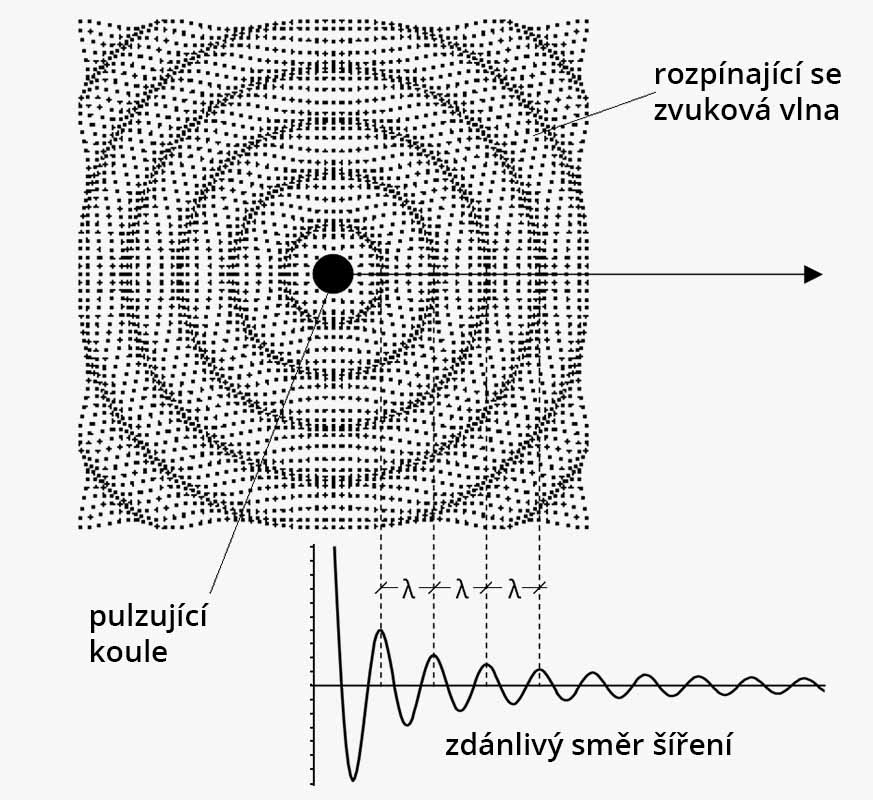
\includegraphics[width=0.5\linewidth]{Obrazky/mic-uni-proximity-fig-2-sound-wave-CZ.jpg}
    \caption{Zvuk šířící se z bodového zdroje\newline
    Zdroj: https://www.audiopro.cz/reseni/co-je-a-jak-se-projevuje-proximity-efekt/}
    \label{fig:enter-label}
\end{figure}
\end{center}



\subsection{Odraz zvuku}
Když zvuk dopadá na stěnu, tak část jeho energie je absorbována zdí a část je emitovaná z jednotlivých bodů zpět do prostoru. Z těchto bodů se zvuk šíří podle zákonu odrazu, který říká, že úhel dopadu je roven úhlu odrazu. To znamená že pokud se zvuk šíří z bodového zdroje, tak odraz zvuku vypadá jako stejná vlna s menší amplitudou, která je osově symetrická vzhledem k dané stěně viz. obrázek č. 2 a 3. \cite{papirNaZvuk}
\begin{figure}
    \centering
    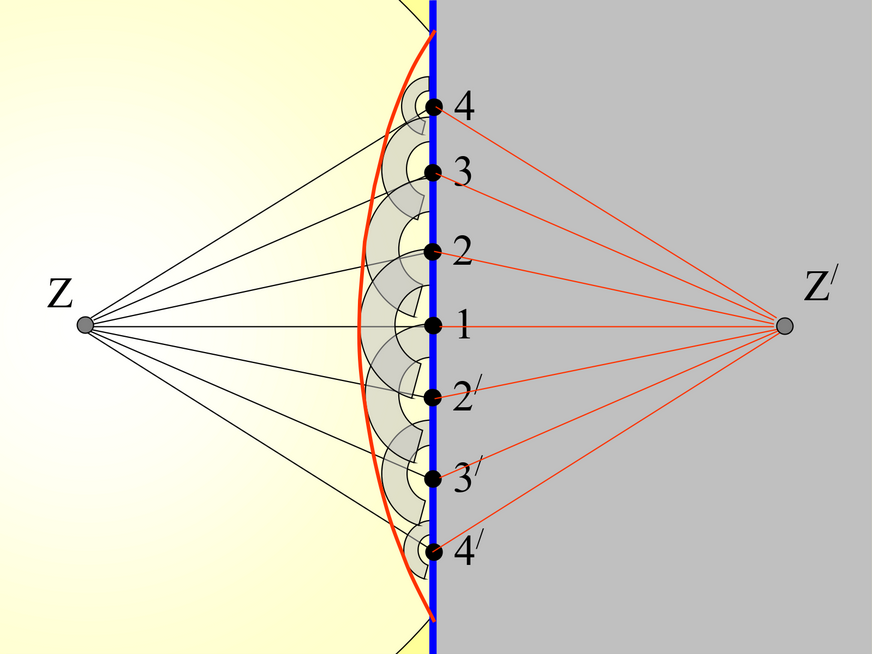
\includegraphics[width=0.5\linewidth]{Obrazky/odraz zvuku s bodama.png}
    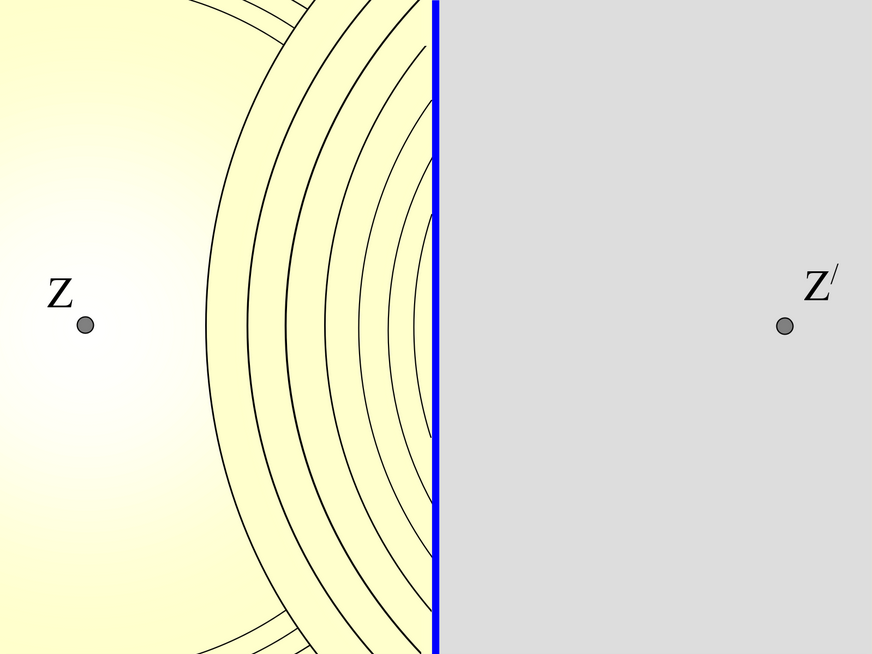
\includegraphics[width=0.5\linewidth]{Obrazky/odraz zvuku bez bodu.png}
    \caption{schema odrazu zvuku s jednotlivými body\\
    Zdroj: Prezentace: Odraz a lom vlnění (PaedDr. Jozef Beňuška  jbenuska@nextra.sk)}
    \label{fig:enter-label}
\end{figure}

\vspace{0.7cm}
\newpage
\section{Obecné popsání programu}
Při spuštění programu se uživateli zobrazí jednoduché a přehledné menu,  na kterém jsou 2 tlačítka: \textit{místnost1} a \textit{místnost2} viz obrázek č. 3, pokud uživatel klikne tlačítko je přesměrován do náležité místnosti. \textit{Místnost1} reprezentuje čtvercový tvar  a \textit{místnost2} reprezentuje více obdelníkový tvar místnosti. Tak je možné pozorovat různé rozdíly v tom, jak se zvuk šíří v místnostech s různými rozměry. 

    \begin{figure}[htpb]
    \centering
    \includegraphics[width=0.5\linewidth]{Obrazky/Hlavní menu.PNG}
    \caption{Hlavní menu \vspace{0.1cm}
    \newline Zdroj: vlastní}
    
    \label{fig:enter-label}
    \end{figure}
Obě místnosti jsou rozděleny na 3 části grafickou strukturou \textit{VBox}. V první části \textit{VBoxu} jsou tlačítka \textit{Stop}, \textit{Resume}, \textit{Reset}. Tlačítko \textit{Stop} simulaci zastaví, \textit{Resume} ji spustí a \textit{Reset} vymaže všechny vlny z obrazovky. Dále je na scéně zobrazen čtverec který má roli místnosti. A nakonec dole na scéně je tlačítko \textit{Hlavni Menu}, které přesměruje uživatele do hlavního menu a časovač, který slouží na časování toho jak dlouho je simulace spuštěná. Časovač  navíc slouží k indikaci, zda program běží plynule, nebo dochází k jeho zasekávání.\newpage 

\begin{figure}[htpb]
    \centering
    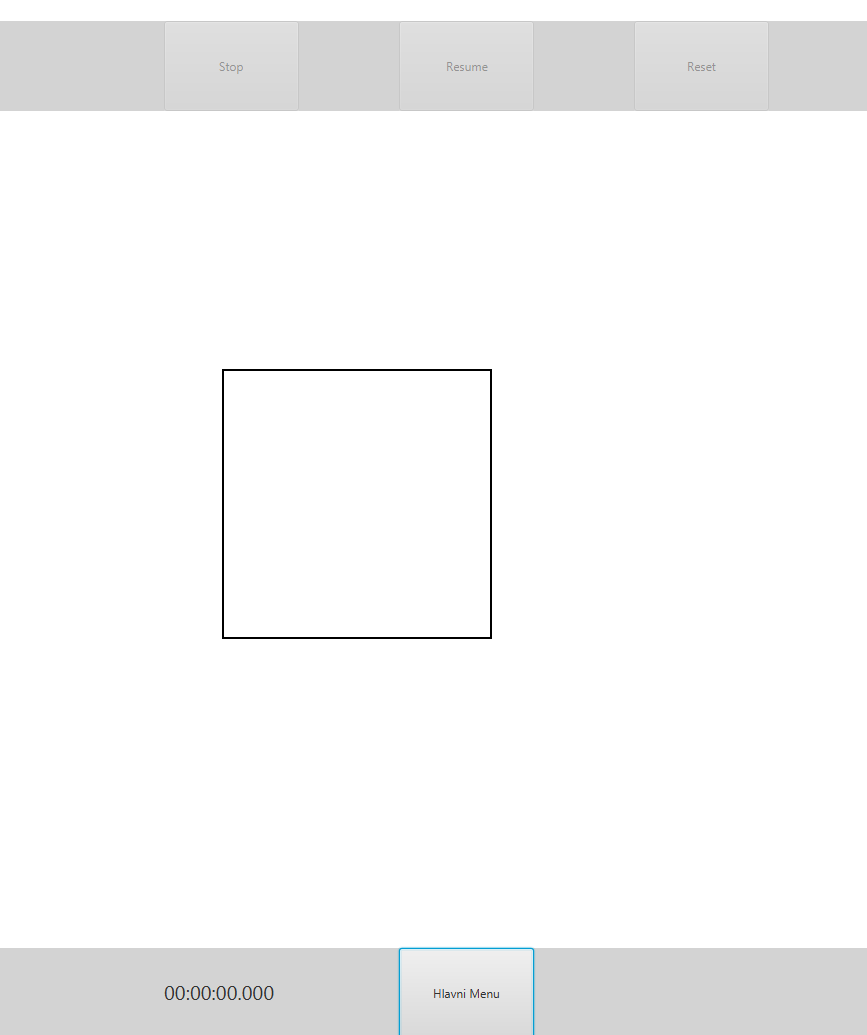
\includegraphics[width=0.7\linewidth]{Obrazky/mistnost0.png}
    \caption{Místnost 1 Zdroj: vlastní}
    \label{fig:enter-label}
\end{figure}

Pokud uživatel klikne do místnosti vytvoří se vizuální reprezentace expandující  zvukové vlny. 

\subsection{Zjednodušení}
Jelikož simulování zvukové vlny je velice náročné na grafický procesor tak bylo nutno vytvořit značně zjednodušený algoritmus, který ale bude simulovat vlnu co nejpřesněji. Mezi tato zjednodušení patří například zanedbání zmenšování amplitudy nepřímo úměrně s druhou mocninou vzdálenosti od počátku vlny. Toto rozhodnutí jsem udělal, protože by se musela počítat druhá mocnina společně s vzdáleností, což je odmocnina a dvě druhé mocniny, stokrát až tisíckrát za sekundu. Dále jsem byl nucen zanedbat počítání okamžíté výchylky v bodě pomocí vzorečku:
\[
y(t) = y_m \sin(2\pi f t + \phi)
\]

\begin{itemize}
    \item \( y_m \) - amplituda
    \item \( f \) - frekvence
    \item \( t \) - čas
    \item \( \phi \) - fáze
\end{itemize}

Rozhodl jsem se tak provést, protože počítání sinu společně s násobením desetinných čísel skoro pro každý \textit{Pixel} v místnosti je také velmi náročné. Místo toho je vlna rozdělena na několik kružnic, z nichž každá přidá či odebere pixelům okamžitou výchylku (viz kapitoly 4.11 a 4.14). To efektivně vytvoří vizuální relativně přesnou vizuální reprezentaci vlny bez toho, aniž by se program zasekával. Také bylo nutno počítat okamžitou výchylku i ostatní hodnoty důležité pro generaci vlny  pouze v integerech/ celých číslech, protože počítání v doublech/ desetinných číslech by také vyústilo v sekání programu. Jelikož je vše počítané v integerech tak ne všechny vlnové délky nebo amplitudy jsou povoleny. Proto jsem se rozhodl tyto hodnoty definovat přímo v kódu jako neměnné konstanty a to na následující hodnoty.

\begin{itemize}
    \item vlnová délka / \textit{deltaR} = 60
    \item amplituda = 100
\end{itemize}

\section{Třídy}
\subsection{Launcher}
Třída \textit{Launcher} je potomek třídy \textit{Application}, která je základní třídou potřebnou k vytvoření JavaFX aplikace. To znamená, že musí mít metodu \textit{start}, která je zodpovědná za samotné spouštění aplikace. Tato třída má pouze dvě metody viz. níže. 

\begin{minted}{java}
         @Override
    public void start(Stage stage) throws IOException {
        MainMenu hlavniMenu = new MainMenu();
        hlavniMenu.setScene(stage);
    }

    public static void main(String[] args) {
        launch();
    }
\end{minted}



\subsection{MainMenu}
Třída \textit{MainMenu} se stará o vytvoření scény a definování její velikosti. Vytvořenou scénu následně zobrazí viz. obrázek 1. Tato třída má pouze jednu metodu \textit{setScene(Stage stage)}, která plní následující:
\begin{itemize}
    \item přiřazení správný \textit{fxml} soubor
    \item vytvořit scénu \textit{hlavniMenu}
    \item vytvořit controller \textit{hlavniMenuController}
    \item předat controlleru velikost scény společně se \textit{stagí}
    \item zobrazit \textit{stage} a scénu
\end{itemize}
\subsection{MainMenuController}
Tato třída slouží jako controller ke třídě \textit{MainMenu}, to znamená že se stará o dynamické aktualizování \textit{VBoxu} (grafické rozhraní) a uživatelské interakce pomocí tlačítek \textit{setSceneDimensions(int height, int width)}, \textit{setStage(Stage stage)}, \textit{updateLayout()}, \textit{handleButtonRoom0Click()} a \\
\textit{handleButtonRoom1Click()}. \newline

\underline{\textbf{\textit{setSceneDimensions(int height, int width)}}}\\
Předává \textit{stage} z třídy \textit{MainMenu} do controlleru. To umožnuje controlleru starat se o změnu \textit{stage} nebo změnu scény.

\vspace{0.3cm}

\underline{\textbf{\textit{updateLayout()}}}\\
Toto je privátní metoda, která je zodpovědná za vypočítávání rozměrů a dynamické aktualizování \textit{VBoxu} vzhledem k velikosti scény. 

\vspace{0.3cm}

\underline{\textbf{\textit{handleButtonRoom0Click()}}}\\
Metoda se zavolá pokud uživatel klikne na tlačítko s názvem \textit{MÍSTNOST 1}. Metoda vytvoří novou instanci třídy \textit{Room0} a přesměruje uživatele na příslušnou scénu. To samé dělá i metoda handleButtonRoom1Click(), s rozdí-lem že tato metoda přesměruje uživatele do jiné místnosti. 
\subsection{Room0 a Room1}
Tyto dvě třídy jsou zodpovědny za inicializaci počáteční velikosti scény, načítání příslušného \textit{FXML} souboru, vytváření a zobrazování  scény a \textit{stage}, vytváření controlleru a připisování controlleru k \textit{fxml} souboru. Třídy mají tři metody \textit{setScene(Stage stage)}, která se stará o vše výše zmíněné, \textit{ getMistnost0ScreenHeight()}, \textit{ getMistnost0ScreenWidth()}. \textit{Room1} vytváří scénu ze 4. obrázku a \textit{Room1} vytváří scénu velmi podobnou s jediným rozdílem a to že místo čtvercové místnosti je tam obdelníková. 

\subsection{BaseRoomControllerInterface}
Interface, který musí implemenovat každý \textit{RoomController}. Implementace je nutná kvůli většímu počtu místností společně s předáváním a získáváním informací ze tříd \textit{SoundWave}, \textit{WaveManager} atd. V interfacu jsou následující metody: \textit{setStage(Stage stage), initialize(), getXMin(), getXMax(), getYMin(), getYMax(), overlayRectangles(), updateLayout(), getRoomWalls(), getRoomCorners() a getStroke()}
\subsection{Room0Controller}
Tato třída se stará o logiku, rozvržení a  interakce se uživatelem. Přiřadí funkci jednotlivým tlačítkám, spravuje časovač a pokud uživatel klikne do místnosti tak pomocí ostatních tříd jako \textit{WaveManager, PixelManager, SoundWave ...} vytvoří novou zvukovou vlnu. Controller má následující metody:

\vspace{0.3cm}  
\underline{\textbf{\textit{setStage(Stage stage)}}} \newline
Nastaví hlavní okno aplikace pro scénu Room0.

\vspace{0.3cm}  
\underline{\textbf{\textit{initialize()}}} \newline 
Inicializuje scénu, UI komponenty a další proměnné (např. stav obdélníku nebo tlačítek) při načtení ovladače.

\vspace{0.3cm}  
\underline{\textbf{\textit{createTimeline()}}}  \newline
Spustí časovač pro správu časově závislých událostí ve scéně.

\vspace{0.3cm}  
\underline{\textbf{\textit{initializeRectangle(double x, double y)}}}  \newline
Nastaví obdélník v místnosti na základě zadaných rozměrů.

\vspace{0.3cm}  
\underline{\textbf{\textit{getXMin(), getXMax(), getYMin(), getYMax()}}}  \newline
Vrátí minimální a maximální souřadnice x/y místnosti pro určení hranic nebo umístění prvků rozvržení.

\vspace{0.3cm}  
\underline{\textbf{\textit{updateLayout()}}}  \newline
Dynamicky upravuje velikost a pozici tlačítek nebo UI komponent místnosti podle jejích rozměrů.

\vspace{0.3cm}  
\underline{\textbf{\textit{createOverlay() a overlayRectangles()}}}  \newline
Odpovídají za vykreslení překrývajícich obdelníků.

\vspace{0.3cm}  
\underline{\textbf{\textit{initializeLines(double xMin, double xMax, double yMin, double yMax)}}}\\
Vytváří nové přímky pomocí třídy \textit{Line}, které reprezentují stěny místnosti. Tyto přímky jsou používány při počítání odrazu vlny, konkrétně k vytvoření vlny symetrické vůči dané stěně. Dále vytvoří seznam těchto přímek \textit{roomWalls} a rohů místnosti \textit{roomCorners}. 
\newpage 
\underline{\textbf{\textit{getRoomWalls()}}}  \newline
Vrátí seznam čar představujících stěny místnosti.

\vspace{0.3cm}  
\underline{\textbf{\textit{getRoomCorners()}}}  \newline
Vrátí seznam bodů představujících rohy místnosti.

\vspace{0.3cm}  
\underline{\textbf{\textit{handleButtonHlavniMenuClick()}}}  \newline
Přepne scénu zpět do hlavního menu.

\underline{\textbf{\textit{handleButtonStopClick()}}}  \newline
Zpracovává uživatelskou interakci k zastavení časovače a vln.

\vspace{0.3cm}  
\underline{\textbf{\textit{handleButtonResumeClick()}}}  \newline
Obnoví pozastavenou aktivitu ve scéně .

\vspace{0.3cm}  
\underline{\textbf{\textit{handleButtonResetClick()}}}  \newline
Obnoví stav místnosti do původního nastavení.

\vspace{0.3cm}  
\underline{\textbf{\textit{updateTimerLabel()}}}  \newline
Tato metoda odpovídá za aktualizování časovače.

\vspace{0.3cm}  
\underline{\textbf{\textit{handlePaneClick(MouseEvent event) }}}  \newline
Zavolá se pokud uživatel klikne na \textit{centerPane}, pokud klikne do místnosti tím je myšleno do vykresleného čtverce tak pomocí třídy \textit{WaveManager} vytvoří zvukovou vlnu. Nejprve se vytvoří animace a potom se volá metoda \textit{updateWaves}  ve třídě \textit{WaveManager}. 
\subsection{Room1Controller}
Třída Room1Controller je velmi podobná třídě Room0controller. Metody: \textit{setStage(Stage stage), initialize(), createTimeline(), getStroke(), getRoomWalls(), getRoomCorners(), getXMin(), getXMax(), getYMin(), getYMax(), initializeLines(double xMin, double xMax, double yMin, double yMax), updateLayout(), createOverlay(), overlayRectangles(), updateTimerLabel(), handleButtonHlavniMenuClick(), handleButtonStopClick(), handleButtonResumeClick(), handleButtonResetClick(), handlePaneClick(MouseEvent event)} plní stejnou funkci jako ve třídě Room0Controller viz. kapitola 4.6. Pouze třída \textit{initializeRectangle(double x, double y)} je rozdílná a to v tom, že místo čtverce se vytvoří obdelník.
\subsection{Line}
Toto je jednoduchá třída, reprezentující přímku v rovině. V programu se používá při reprezentaci stěn a při výpočtu odrazu vlny. Třída má  3 atributy \textit{A, B, C}, které značí hodnoty v obecné rovnici přímky:\\
\[
Ax + By + C = 0
\]
Ve třídě je konstruktor, kde se hodnoty nastaví a potom 3 \textit{gettery}, z nichž každý vrací právě jednu hodnotu (\textit{A, B} nebo \textit{C}).
\subsection{Point} 
\textit{Point} je třída která reprezentuje bod rovině. Má 2 atributy \textit{x} a \textit{y}, ty značí souřadnice na scéně, které fungují stejně jako souřadnice v kartézské souřadnicové soustavě. Tudíž se zde mohou používat stejné výpočty jako v analytické geometrii. \\
Jelikož má třída dva konstruktory, tak je možné instanci této třídy inicializovat dvěma způsoby. První způsob je pomocí zadání samotných souřadnic a druhý je pomocí průsečíku dvou přímek (\textit{Line}). Průsečík počítá třída Calculator, která je popsána v kapitole 4.10. 
Dále má třída následující metody: \textit{getX(), getY(), setX(double x), setY(double y), toString(), distance(Point other)}.

\subsection{Calculator}
\textit{Calculator} je třída, která vypočívává souřadnice bodů. Má dvě metody: \textit{calculateIntersection(Line line1, Line line2)}\cite{pruseciky}, která zjistí souřadnice průsečíku dvou přímek a \textit{calculateSymetricPoint(Point point, Line line)}\cite{symetrie}, jenž zjistí souřadnice osově souměrného bodu vůči danné přímce. Obě metody vrací \textit{Point} a vypadají následovně:\\
\footnotesize
\begin{minted}{java}
    public Point calculateIntersection(Line line1, Line line2) {
        // Extract coefficients from each line
        double A1 = line1.getA();
        double B1 = line1.getB();
        double C1 = line1.getC();
        double A2 = line2.getA();
        double B2 = line2.getB();
        double C2 = line2.getC();
        // Calculate determinant
        double determinant = A1 * B2 - A2 * B1;
        // If determinant is 0, the lines are parallel or coincident
        if (determinant == 0) {return null;}
        // Calculate the intersection point
        double x = (B1 * C2 - B2 * C1) / determinant;
        double y = (A2 * C1 - A1 * C2) / determinant;
        return new Point(x, y);
    }
    public Point calculateSymetricPoint(Point point, Line line){
        // Extract line coefficients
        double A = line.getA();
        double B = line.getB();
        double C = line.getC();
        // Extract point coordinates
        double x = point.getX();
        double y = point.getY();
        // Calculate projection point
        double denominator = A * A + B * B;
        if (denominator == 0) {throw new IllegalArgumentException("Invalid 
        line coefficients:A and B cannot both be zero.");}
        double x_proj = (B * (B * x - A * y) - A * C) / denominator;
        double y_proj = (A * (-B * x + A * y) - B * C) / denominator;
        // Calculate symmetric point
        double x_sym = 2 * x_proj - x;
        double y_sym = 2 * y_proj - y;
        // Return the symmetric point
        return new Point(x_sym, y_sym);
    }
\end{minted}
\normalsize





\subsection{Pixel}
Třída \textit{Pixel} znázorňuje zvětšený individuální pixel v místnosti. Je  potomkem třídy \textit{Rectangle} to proto, aby byla jednoduchá změna barvy či přidávání na scénu. 
Třída má následující atributy:
\begin{itemize}
    \item \textit{gridX/Y} -  pozice v gridu neboli 2D poli místnosti 
    \item \textit{realX/Y} -  reálná pozice na scéně
    \item \textit{celkovaVychylka} -  celková výchylka v bodě
    \item \textit{PIXELSIZE} - velikost pixelu
    \item \textit{rectangle} - vizuální reprezentace pixelu
\end{itemize}

Celkem má třída 8 metod, z nichž každá plní specifickou funkci.\\

\textbf{\textit{setPixelSize(int pixelSize)}}\\
Nastaví velikost pixelu.

\vspace{0.3cm}
\textbf{\textit{getGridY/X(double realY/X, double y/xMIn)}}\\
Vrátí hodnoty \textit{gridX/Y}. 

\vspace{0.3cm}
\textbf{\textit{getRectangle()}}\\
Vrátí samotní obdelník.

\vspace{0.3cm}
\textbf{\textit{setColor(int celkovaVychylka)}}\\
Přiřadí barvu vzhledem k velkové výchylce.

\vspace{0.3cm}
\textbf{\textit{setDefault()}}\\
Nastaví celkovou výchylku na 0.

\vspace{0.3cm}
\textbf{\textit{addVychylka(int vychylka)}}\\
Přidá výchylku do celkové výchylky.

\vspace{0.3cm}
\textbf{\textit{createColor(int celkovaVychylka)}}\\
Přiřadí barvu k celkové výchylce pomocí if - elseif řetězce. Pokud je celková výchylka menší než -20 tak metoda vrátí modrou barvu (čím je to menší tím je modrá víc sytá), když je celková výchylka větší než 20 tak metoda vrátí červenou (čím je výchylka větší tím je červená sytější) a pokud je hodnota mezi -20 a 20 tak se vrátí bílá barva. Metoda přiřadí výchylku do intervalu od 400 do -400. Podle toho jak velká výchylka bude, tak se ji přiřadí příslušná barva.

\vspace{0.3cm}
\textbf{\textit{getCoordinates()}}\\
Vrátí instanci třídy \textit{PixelCoordinate} se souřadnicemi pixelu viz. kapitola 4.12.

\subsection{PixelCoordinate}
Toto je pomocná třída, která slouží pouze jako nástroj pro ukládání souřadnic pixelů v gridu. Má 2 atributy\textit{ x} a \textit{y}, ty slouží jako souřadnice. Dále má třída 2 \textit{gettery} každý buď pro \textit{x} nebo \textit{y}, metodu \textit{equals(Object obj)}, která se používá při lokaci duplikátů v algoritmu na přiřazování pixelů dané kružnici viz. kapitola 4.14. Jako poslední metoda, kterou tato třída má je \textit{hashCode()}, jenž se také používá při lokaci duplikátů.
\subsection{PixelManager}
Tato třída slouží ke spravování celého 2D pole pixelů. Mezi její funkce patří například inicializace pole, aktualizování jednotlivých pixelů nebo resetování všech neaktivních pixelů. Mezi klíčové atributy patří: 
\begin{itemize}
    \item \textit{Pixel[ ][ ] pixelGrid} - představuje 2D pole pixelů v místnosti
    \item \textit{int width} - šířka pole
    \item \textit{int height} - výška pole
    \item \textit{BaseRoomControllerInterface roomController} - zpřístupňuje metody a proměnné z jednotlivých controllerů např. \textit{Pane centerPane} 
    \item \textit{int PIXELSIZE} - konstanta reprezentující velikost jednoho pixelu
\end{itemize}
Třída má celkem 6 metod.\\
\\
\textbf{\textit{initializePixelGrid(int rectWidth, int rectHeight, double rectX, double rectY)}}\\
Tato metoda inicializuje \textit{pixelGrid}, to znamená, že se připíšou jednotlivé pixely na správně pozice do místnosti i do \textit{pixelGridu}. Metoda se volá ve třídách \textit{Room0/1Controller}, konkrétně v metodě \textit{initializeRectangle}.\\
\\
\textbf{\textit{addRectanglesToPane(Pane pane)}}\\
Přidá všechny pixely na scénu pomocí \textit{pane}. Je také použita ve třídách \textit{Room0/1Controller} v metodě \textit{initializeRectangle}.\\
\\
\textbf{\textit{resetPixelGridDisplacement()}}\\
Zodpovídá za resetování všech pixelů. To znamená, že pro každý pixel zavolá metodu \textit{setDefault()}. Metoda se volá v \textit{Room0/1Controllerech} v metodě \textit{handleButtonResetClick()}.\\
\\
\textbf{\textit{resetAllInactivePixels(Set activePixelCoordinates)}}\\
Účel této metody je resetování všech pixelů, které nejsou momentálně v žádné vlně. Metoda projde celý \textit{pixelGrid} a pro každý pixel získá jeho \textit{PixelCoordinate} a zjistí zda jsou dané souřadnice napsané v setu \textit{activePixelCoordinates}. Pokud jsou, tak se nic neděje a pokud nejsou, je daný  pixel vynulován (zavolá se metoda \textit{setDefault()})\\
\\
\textbf{\textit{getPixelSize(), getPixelGrid()}}\\
Slouží jako \textit{gettery} pro \textit{PIXELSIZE} a \textit{pixelGrid}.

\subsection{SoundWave}
\textit{Soundwave} je potomkem třídy \textit{Circle} a reprezentuje individuální expandující zvukovou vlnu. Zvuková vlna má tvar expandujícího torusu/donutu, který je znázorněn jako oblast mezi vnějším a vnitřním kruhem (\textit{outerCircle} a \textit{innerCircle}). Třída také interaguje s \textit{pixelGridem} pomocí třídy \textit{PixelManager} a \textit{WaveManager} a zjišťuje, jakým pixelům má přidat výchylku. Dále zjišťuje body a momenty odrazu vlny a způsobuje samotnou expanzi. Jelikož je třída velmi obsáhlá (cca 500 řádků kódu a 30 metod), tak zde není popsaná každá metoda zvlášť jako u předchozích tříd, ale je popsaná jen logika.  \\



\subsubsection{Inicializace}
Nová vlna se vytvoří, pokud uživatel klikne do místnosti, nebo se vlna odrazí od zdi. Když se tvoří nová instance, tak se nejprve zavolá konstruktor, který nastaví střed (vytvoří se \textit{Point} se souřadnicemi středu), poloměr, controller, stěny místnosti (xMin/Max a yMin/Max), časovač, osy kružnice, tj. 2 přímky (\textit{Line} viz. kapitola 4.8), rohy místnosti a body, kde se vlna odrazí od stěn.\\
Body odrazu se hledají jako průsečíky os kružnice a stěn místnosti. Používá se k tomu metoda \textit{getIntersections()}. Tato metoda zjistí, kde se nachází střed vlny a pomocí třídy \textit{Calculator} najde již zmíněné průsečíky. Průsečíky se vrátí jako pole \textit{Pointů}, toto pole je klíčové k počítání odrazu vlny. 



\subsubsection{Expanze}
O expanzi vlny se stará metoda \textit{grow()}. Tato metoda nejprve zvětší poloměr vnější kružnice \textit{outerrRadius} o 1, potom zjistí, jesli je větší než \textit{deltaR} (rozdíl poloměru vnitřního a vnějšího kruhu) neboli délka zvukové vlny. Jestliže je větší, tak zkontroluje zda existuje vnitřní kruh, pokud ne tak se vnitřní kruh vytvoří a pokud ano tak se poloměr vnitřního kruhu \textit{innterRadius} také zvětší o 1.\\
Dále se zkontroluje jestli je \textit{outerRadius} dělitelný \textit{PIXELSIZE} a zároveň simulace běží, pokud jsou tyto podmínky splněny, tak se vymažou hodnoty ze setu \textit{savedSetOfPixelCoords}, zavolá se metoda \textit{generateWaveDonut()} (viz. kapitola 4.14.4) a hodnoty ze setu \textit{activePixelCoordinates} se přepíšou do setu \textit{savedSetOfPixelCoords}. Nakonec se zavolá metoda \textit{resetVisitedPixels()}, která vymaže všechny hodnoty ze setů 
\textit{visitedPixels, duplicatePixels, activePixelCoordinates}.

\begin{figure}[htpb]
    \centering
    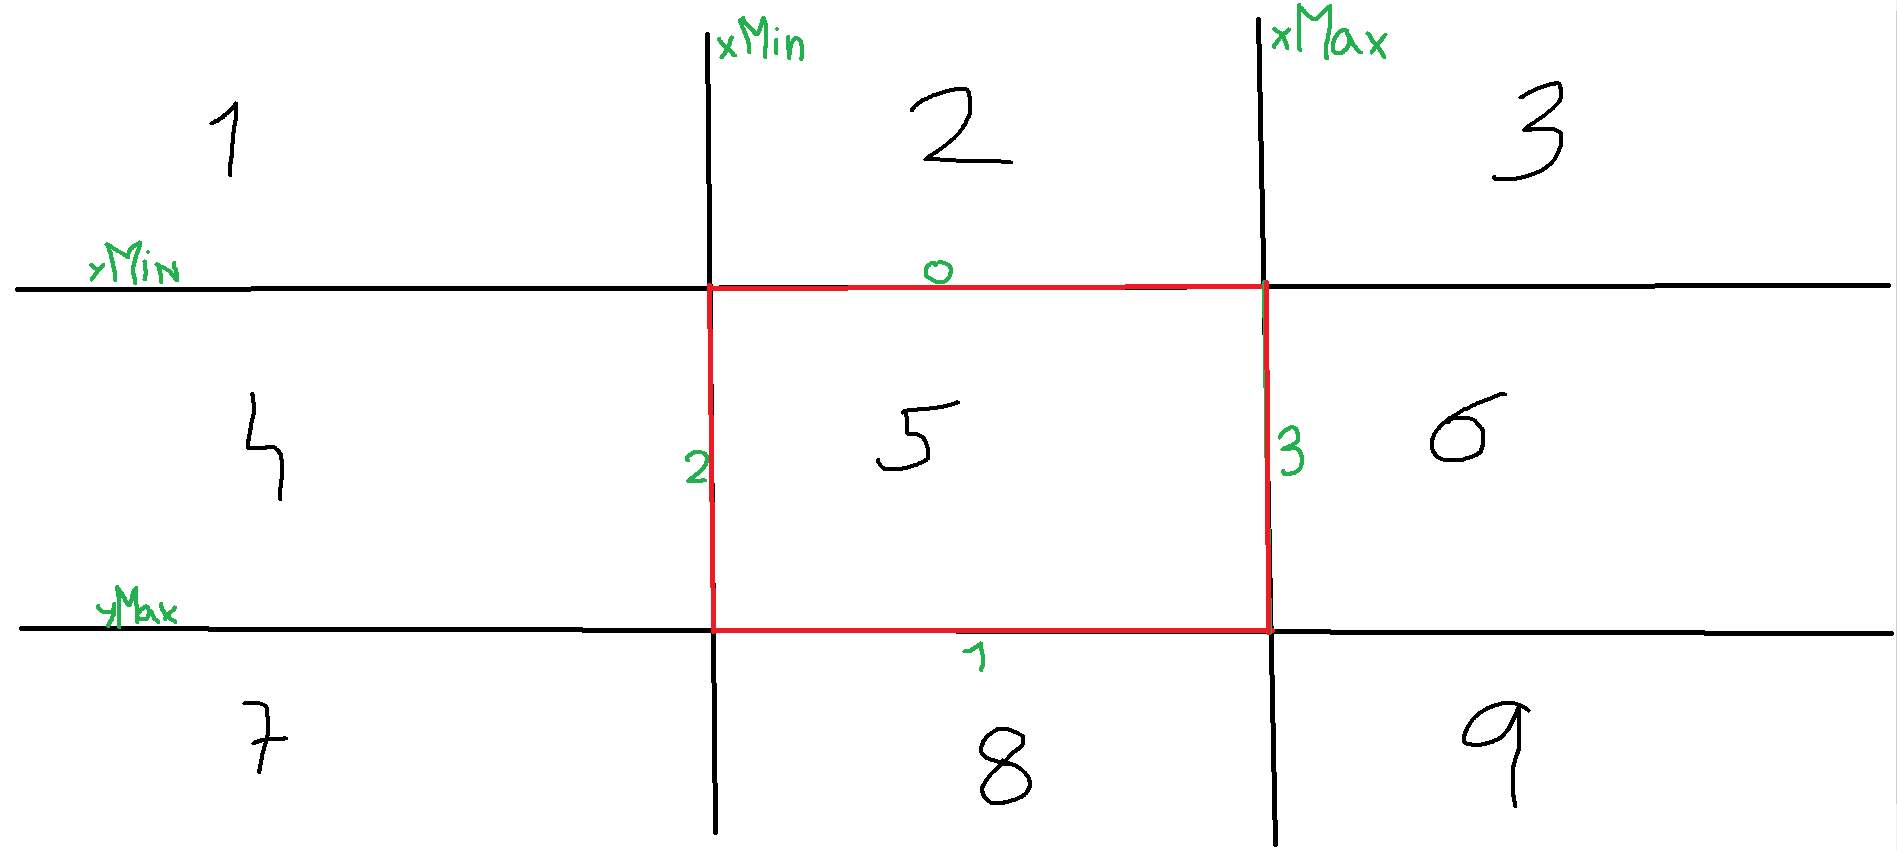
\includegraphics[width=0.7\linewidth]{Obrazky/Schema mistnosti.png}
    \caption{Schéma místností Zdroj: vlastní}
    \label{fig:enter-label}
\end{figure}


\subsubsection{Odstraňování}
Vlna se odstraní pokud je její amplituda menší než nula nebo je starší než \textit{maxAge} (8 sekund). \textit{maxAge} byl zvolen jako 8 sekund, protože tolik trvá \textit{innerCircle},  než se expanduje pryč z místnosti.

\subsubsection{Odraz}
Zvuková vlna se odrazí, pokud se dotkne stěny. Tato logika v programu funguje následovně. Nejprve se zjistí, při jakých poloměrech se vlna odrazí od zdi, neboli jak moc je vlna vzdálená od každé zdi. Tyto vzdálenosti najde metoda \textit{getReflectionDistances}, která vrací pole celých čísel / integerů. Nejdříve metoda zjistí v jakém sektoru scény (viz. obrázek 5) leží pomyslný střed (v případě kdy je vlna vytvořena kliknutím uživatele, tak reálný střed). Vlna se může nacházet v devíti různých sektorech 1-9, které tvoří 3 logicky podobné skupiny (první je 5, druhá je 2,4,6,8 a třetí je 1,3,7,9). Skupiny jsou si podobné tehdy když mají osy vlny v daných skupinách stejný počet průsečíku se stěnami místnosti. Pro první skupinu jsou průsečíky 4, pro druhou je jeden a pro třetí je jich 0.
To, jestli střed leží v daném sektoru, zjišťují metody: \textit{isInRectangle, isBellowRectangle,isAboveRectangle, isLeftOfRectangle, isRightOfRectangle, isAboveOnTheRightOfRectangle, isAboveOnTheLeftOfRectangle, isBellowOnTheRightOfRectangle, isBellowOnTheLeftOfRectangle}. Tyto metody vrací boolean a jsou použity jako podmínky v if-else if řetězci v metodě \textit{getReflectionDistances}.\\
Jako první a nejjednodušší na počítání je sektor 5, střed vlny je reálný a nachází se v místnosti. Vzdálenosti se tehdy určují pouze jako vzdálenosti průsečíků os se stěnami a středem. Tyto vzdálenosti jsou 4 tím pádem metoda vrátí pole integeru o velikosti 4. Dále s těmito vzdálenostmi pracuje třída \textit{WaveManager}.\\
Pro druhou skupinu neboli sektory 4,8,6,8 se ve třídě \textit{SoundWave} počítá pouze jedna vzdálenost a to ta od středu k průsečíku opačné strany. V tomto případě metoda vrací pole o velikosti 1 s danou vzdáleností, ostatní vzdálenosti počítá třída \textit{WaveManager}.\\
Třetí skupina se počítá jinak než první 2. Jelikož je střed vlny diagonálně od místnosti, tak osy vlny nemají se stěnami místnosti žádný průsečík, proto je zde potřeba uplatnit jiný výpočet odrazových vzdáleností. Protože se vlna šíří jakoby z rohu místnosti, tak se vždy dotkne první rohů opačných stěn. Takže je nutné vypočítat pouze vzdálenosti k ostatním rohům místnosti. Počet těchto vzdáleností je 3 takže metoda vrací pole o velikosti 3. 

\subsubsection{Vykreslování}
Zvuková vlna má tvar donutu, tento tvar program chápe jako prostor mezi vnějším (\textit{ounterCircle}) a vnitřním kruhem (\textit{innterCircle}). Prostor je rozdělen na 20 ( včetně \textit{innerCircle} a \textit{outerCircle}) podkružnic. Počet těchto podkružnic je roven podílu velikosti pixelu (\textit{PIXELSIZE}) a vlnové délky / rozdílu poloměru vnějšího a vnitřního kruhu (\textit{deltaR}). \\
Každá z těchto podkružnic zvýší nebo sníží celkovou výchylku daného pixelu o \textit{amplituda/5}. Prvních 5 ji zvýší, druhých 10 ji sníží a zbytek ji zvýší. Toto vytvoří iluzi sinusoidy s jednoduchou a velmi efektivní implementací v kódu. Konkrétně to funguje následovně.\\ 
Pokaždé když se zavolá metoda \textit{grow()} a \textit{outerRadius} je dělitelný \textit{PIXELSIZE}, tak se volá metoda \textit{generateWaveDonut()}. Tato metoda nejprve vypočítá aktuální délku vlny (\textit{width}) a potom vypočítá celkový počet kruhů (\textit{numberOfCircles}), ten se spočítá jako podíl délky vlny a \textit{PIXELSIZE}. Následovně je spuštěn for-cylkus, který běží od nuly do \textit{numberOfCircles}. V tomto for-cyklu se nejprve vypočítá poloměr momentální podkružnice,
\begin{minted}{java}
int radius = innerRadius + ((numberOfCircles - i-1) * PIXELSIZE)
\end{minted}
potom její okamzitaVychylka (\textit{amplitudeForCirrcle}) pomocí metody \textit{calculateAmplitudeForCircle(int circleIndex)}. Tato metoda vrátí buď \textit{amplitude/5}, pokud je index menší než 5 nebo větší než 15, nebo 
\textit{-amplitude/5,} pokud je hodnota indexu jiná. \\
Dále se zavolá metoda \textit{drawCircleWithOkamzitaVychylka(int centerX, int centerY, int radius, int okamzitaVychylkaValue)}\cite{algoritmus}. Tato metoda použije Bresenhamův algoritmus na vykreslování kružnic a zjistí na jakých pixelech (reálné celočíselné pixely na obrazovce) momentálně kružnice leží. 
\begin{minted}{java}
    int x = 0;
    int y = radius;
    int d = 3 - 2 * radius;
    //finds the coordinates of pixels
    while (y >= x) {
        if (d > 0) {
            y--;
            d = d + 4 * (x - y) + 10;
        } else {
            d = d + 4 * x + 6;
        }
        // Set the pixels for this circle
        setCirclePixelsDisplacement
        (centerX, centerY, x, y, okamzitaVychylkaValue);
        x++;
    }
\end{minted}
Hodnoty jsou předány metodě \textit{setCirclePixelsDisplacement(int centerX, int centerY, int x, int y, int okamzitaVychylkaValue)}, která zjistí zda je daná souřadnice v místnosti. Jelikož Bersenhamův algoritmus funguje na bázi kopírování pixelů symetricky podle středu a os symetrií, tak je potřeba zjistit zda se daný pixel nachází v místnosti. To metoda rozpozná za pomoci 8 podmínek (8 protože kruh je symetrický po 8 osách). Zde je příklad několika z těchto podmínek. 
\begin{minted}{java}
if (centerY + y > yMin && centerY + y < yMax &&
    centerX + x > xMin && centerX + x < xMax)
if (centerY + y > yMin && centerY + y < yMax &&
    centerX - x > xMin && centerX - x < xMax)
if (centerY - y > yMin && centerY - y < yMax &&
    centerX + x > xMin && centerX + x < xMax)
if (centerY - y > yMin && centerY - y < yMax &&
    centerX - x > xMin && centerX - x < xMax)
\end{minted}
Pokud se tyto podmínky splní, tak se zavolá metoda setPixelDisplacement(int x, int y, int okamzitaVychylkaValue), jenž přidá okamžitou výchylku kruhu na jednotlivé pixely. Jako první se konvertují souřadnice na scéně na souřadnice v \textit{pixelGridu} pomocí metody \textit{getGridX/Y} ze třídy Pixel. Dále se zkontroluje, zda jsou gridové souřadnice validní a pokud jsou, tak se vytvoří nová instance třídy \textit{PixelCoordinate} \textit{ pixelCoord} se souřadnicemi \textit{gridX/Y}. Poté se zkontroluje, zda daný \textit{pixelCoord} nebyl už jednou přidaný, to znamená jestli není v setu \textit{visitedPixels}. Pokud je tak se přidá do setu \textit{duplicatePixels}, a pokud není, tak se přidá do setů \textit{visitedPixels} a \textit{activePixelCoordinates}, a  \textit{Pixelu} se stejnými souřadnicemi v \textit{pixelGridu} se přidá \textit{okamzitaVychylka} kružnice.  



\subsection{WaveFactory}
Tato třída má funkci továrny na vlny. Má pouze jednu metodu \textit{createWave(double x, double y, BaseRoomControllerInterface controller, int radius, int amplitude, int direction)}, která vrátí novou instanci třídy \textit{SoundWave}.
\subsection{WaveManager}
Třída \textit{WaveManager}, jak z názvu vyplývá, funguje jako manažer pro všechny vlny na scéně. Stará se o aktualizaci scény nebo vytváření, odstraňování a odrazy vln. Dále je zodpovědná za zastavování, spouštění a resetování simulace když uživatel klikne na příslušná tlačítka.

\subsubsection{Vytváření}
K vytvoření individuální vlny se používá metoda \textit{createWave(double x, double y, BaseRoomControllerInterface controller, int radius, int amplitude)}. Metoda nejdříve zkontroluje jeslti je \textit{centerPane} null a pokud není, tak se vytvoří nová vlna pomocí třídy \textit{WaveFactory}. Poté se připíše to \textit{Arraylistu activeWaves} a  přiřadí se jí instance třídy \textit{PixelManager}. 

\subsubsection{Aktualizace scény}
Pro aktualizaci se používá metoda \textit{updateWaves(BaseRoomControllerInterface controller)}. Tato metoda nejdříve vytvoří \textit{ArrayList wavesToRemove} a \textit{HashSet activePixelCoordinates}. Tyto datové struktury slouží na zapisování vln, které je potřeba odstranit a ke sledování \textit{Pixelů}, jenž jsou momentálně ve vlně. Dále se spustí for-cyklus iterující přes každou \textit{SoundWave} v \textit{activeWaves}. Pro každou z těchto vln se nejprve zavolá metoda \textit{grow()}, poté se zkontroluje zda je starší než 8 sekund a jestli je její amplituda  nižší nebo rovna nule. Pokud se tyto podmínky naplní, tak se vlna přiřadí do \textit{Arraylistu wavesToRemove} .  Následně se do \textit{activePixelCoordinates} přidají všechny pixely dané vlny pomocí metody \textit{wave.getactivePixelCoordinates()}. \\
Potom, co se for-cylkus ukončí, tak se vynulují všechny pixely, které nejsou v žádné vlně,  zavolá se metoda \textit{checkWavesForReflections\\(BaseRoomControllerInterface controller)} (viz. kapitola 4.16.3) a smažou se všechny vlny, jenž jsou ve \textit{wavesToRemove}.


\subsubsection{Odraz}
Pokaždé když se aktualizuje scéna pomocí metody \textit{updateWaves()}, tak se zavolá metoda checkWavesForReflections(BaseRoomControllerInterface controller).\\
\\
\textbf{\textit{checkWavesForReflections(BaseRoomControllerInterface\\
controller)}}\\
Tato metoda znovu iteruje přes všechny vlny \textit{wave} v \textit{activeWaves}.  Nejdříve vytvoří  nový \textit{Point center}, který je stejný jako střed vlny. Potom program zkontroluje zda je \textit{center} v místnosti. Pokud je, tak se z vlny získají \textit{reflectionDistances} a spustí se for-cylkus, jenž iteruje přes všechny tyto vzdálenosti. Pokud se \textit{outerRadius} vlny rovná některé z těchto vzdáleností, tak se vytvoří nová přímka reprezentující danou stěnu, následně se pomocí třídy \textit{Calculator} vytvoří symetrický bod, jenž reprezentuje střed nové vlny a nakonec se vytvoří nová vlna s počátečním poloměrem \textit{outerRadius} a amplitudou o 50 menší.\\
Pokud střed vlny neleží v místnosti, tak se zavolá metoda \textit{handleOutOfRectangleWave(SoundWave wave, Point center, BaseRoomControllerInterface controller)}.\\
\\
\textbf{\textit{\textit{handleOutOfRectangleWave(SoundWave wave, Point center, \\BaseRoomControllerInterface controller)}}}\\
Tato metoda zpracovává vlny, jejichž střed neleží v místnosti a funguje následovně.
Nejdříve se z dané vlny získají \textit{reflectionDistances}, dále se zavolají metody \textit{handleOutOfRectangleWaveForCorners(wave, center, controller) a handleDiagonalWavesForCorners(wave, center, controller)}, které zpracová-vají vzdálenosti ke středům (viz další odstavce), potom se zkontroluje, zda je střed vlny ve správné pozici a má správný poloměr. Zde je příklad těchto podmínek
\begin{minted}{java}
if(wave.isAboveRectangle(center.getX(), center.getY()) &&
currentRadius == reflectionDistances[0]){...}
else if (wave.isBellowRectangle(center.getX(), center.getY()) &&
currentRadius == reflectionDistances[0]){...}
\end{minted}

Jestliže jsou tyto podmínky splněny, tak se zavolá metoda \textit{reflectWave} (viz další odstavce), která vytvoří novou symetrickou vlnu.\\
\textbf{\textit{\\handleOutOfRectangleWaveForCorners(SoundWave wave, Point center, BaseRoomControllerInterface controller)}}\\
Tato metoda se specializuje na odraz vln, které mají středy v sektorech 2,4,6,8 (viz. obrázek 5). Nejprve se zjistí, v jakém z těchto sektorů se střed nachází. Poté se zjistí, zda se \textit{outerRadius} rovná vzdálenosti od středu k některému z rohů a pokud ano tak se zavolá metoda \textit{reflectWave}, která vytvoří novou vlnu symetrickou vůči správné zdi. \\
\\
\textbf{\textit{handleDiagonalWavesForCorners(wave, center, controller)}}\\
Tato metoda se stará o odrazy vln, jejichž středy leží v sektorech 1,3,7,9 (viz. obrázek 5). V této metodě se nejprve inicializují rohy místnosti a poloměr \textit{topLeft, bottomLeft, bottomRight, topRight, currentRadius}. Dále se zjistí v jakém sektoru střed leží. Pokud leží v sektoru jedna, tak se počítají vzdálenosti pouze k \textit{bottomLeft, bottomRight, topRight}  a analogicky je to i se středy v ostatních sektorech.  Jakmile se lokalizuje sektor, tak program zkontroluje, zda se \textit{outerRadius} rovná vzdálenosti středu k některému z rohů místnosti, jestli ano tak se vytvoří příslušná symetrická vlna pomocí metody\textit{ reflectWave}.  Zde je příklad jak taková podmínka vypadá. 
\begin{minted} {java}
if (wave.isAboveOnTheLeftOfRectangle(center.getX(),
center.getY())) {
    if (currentRadius== 
    (int)wave.getCenter().distance(bottomLeft)){
        reflectWave(wave, controller, 1);
    }
    if (wave.getRadius() == 
    (int)wave.getCenter().distance(bottomRight)) {
        Point pomocnyBod = 
        calculator.calculateSymetricPoint
        (center,controller.getRoomWalls().get(1));
        reflectWave(pomocnyBod,
        wave.getOuterRadius(), controller, 3, wave.getAmplitude());
    }
    if (currentRadius==
    (int) wave.getCenter().distance(topRight)){
        reflectWave(wave, controller, 3);
    }

\end{minted}
\vspace{2cm}
\textbf{\textit{reflectWave(SoundWave wave, BaseRoomControllerInterface controller, int wallIndex)}}\\
Tato metoda se stará o vytváření odražených vln s pomocí \textit{SoundWave, BaseRoomControllerInterface a wallIndex}.  Nejprve se inicializuje střed vlny a  přímka, jenž reprezentuje stěnu, od které se vlna odráží. Poté se za pomoci třídy \textit{Calculator} vytvoří symetrický bod \textit{symetricPoint} a vytvoří se nová vlna se středem v symetrickém bodě, počátečním poloměrem \textit{outerRadius} a amplitudou o 50 menší. Metoda \textit{reflectWave(Point center, int currentRadius, BaseRoomControllerInterface controller, int wallIndex, int amplituda)} dělá úplně to samé jen za pomoci jiných parametrů.\\
\\
Třída \textit{WaveManager} má také metody \textit{resumeWaves(), pauseWaves(), resetWaves()}, tyto metody bud zastaví, znovu spustí nebo resetují animaci. Poslední metoda, kterou tato třída obsahuje, je  \textit{removeAllWaves(Pane centerPane)}. Ta odstraní všechny vlny ze scény.
\newpage
\section{Závěr}
Jako ročníkový projekt jsem si vybral simulování zvuku, protože jsem předpokládal, že to bude velmi zajímavé. Při programování jsem pochopil, jak se pohybuje zvuk v místnosti a také jsem poprvé musel pracovat na efektivitě, aby program dobře fungoval. Zjistil jsem, že JavaFX  je hodně špatný framework  na tvoření dynamických simulací, protože všechny operace dělá velmi pomalu oproti ostatním programovacím jazykům. \\
I přes všechna nutná zjednodušení, program splňuje zadání a správně vizuálně reprezentuje, jak se impulzy zvuku pohybují v místnosti. Celkem program zvládne simulovat dvě vlny zároveň, pokud uživatel přidá na scénu více vln, začne se program sekat a ne všechny pixely se budou přepisovat správně.  \\
Ve výsledku mě programování této aplikace velmi bavilo a všechny problémy, na které jsem narazil, se mi podařilo vyřešit s menšími či většími potížemi. 

\newpage
\listoffigures


\newpage
    \bibliographystyle{abbrv}
    \bibliography{Reference.bib}
    \newpage
    
\end{document}
